\section{4. Лемма Даламбера. Основная теорема алгебры (схема доказательства).}

\begin{reminder}
    $e^{i\phi} = \cos(\phi) + i\sin(\phi)$.
\end{reminder}

\begin{lemma}[Д'Аламбера]
    \label{lemma6}
    Пусть $f(x)$ -- многочлен положительной степени из кольца $\Cm[z]$ и $f(z_0) \neq 0$. Тогда $\forall U_{\varepsilon}(z_0)$ найдется $z \in U_{\varepsilon}(z_0)$, такое что $|f(z)| < |f(z_0)|$.
\end{lemma}

\begin{proof}
    Зафиксируем $\varepsilon > 0$. Разделим $f(z)$ на $z - z_0$ с остатком: $f(z) = q_1(z) (z-z_0) + r_0$. Мы знаем, что остаток имеет смысл значения многочлена в точке $z_0$, то есть $r_0 = f(z_0)$. Разделим теперь $q_1$ на $z - z_0$ и подставим полученное выражение в выражение для $f$ (здесь $r_1 = q_1(z_0)$). Получаем 
    $f = q_2(z)(z-z_0)^2 + r_1(z-z_0) + r_0$. Продолжим разложение и получим
    $f(z) = f(z_0) + \frac{f'(z_0)}{1!}(z - z_0) + \frac{f''(z_0)}{2!}(z - z_0)^2 + \dots$ (здесь $r_0 = f(z_0), r_1 = f'(z_0), \ldots, r_k = \frac {f^{(k)}(z_0)}{k!}$). Такое разложение напоминает разложение в ряд Тейлора.
    Обозначим главную часть за $\alpha (z - z_0)^p$, $\alpha \neq 0$, $p \in \N$. Получим
    $f(z) = f(z_0) + \alpha (z-z_0)^p + o((z-z_0)^p)$.
    $f(z) = f(z_0) + (z - z_0)^p \left( \alpha + \frac{o((z-z_0)^p)}{(z-z_0)^p} \right)$, где $o((z - z_0)^p) \vdots (z - z_0)^p$. Так как последнее частное стремится к 0 при $z$, стремящимся к $z_0$, то верно
    $$\exists \varepsilon_1 < \varepsilon \ \forall z \in U_{\varepsilon_1}(z_0) \hookrightarrow \left| \frac {o((z-z_0)^p)}{(z-z_0)^p} \right| < \frac {|\alpha |}{2}.$$
    $$arg \alpha - \frac {\pi}{6} \leq arg(\alpha + \frac {o((z - z_0))^p}{(z - z_0)^p}) \leq arg \alpha + \frac {\pi}{6}, \ \alpha \in \left[\alpha_0, \alpha_0 + \frac {\pi}{3}\right].$$
    \begin{center}
        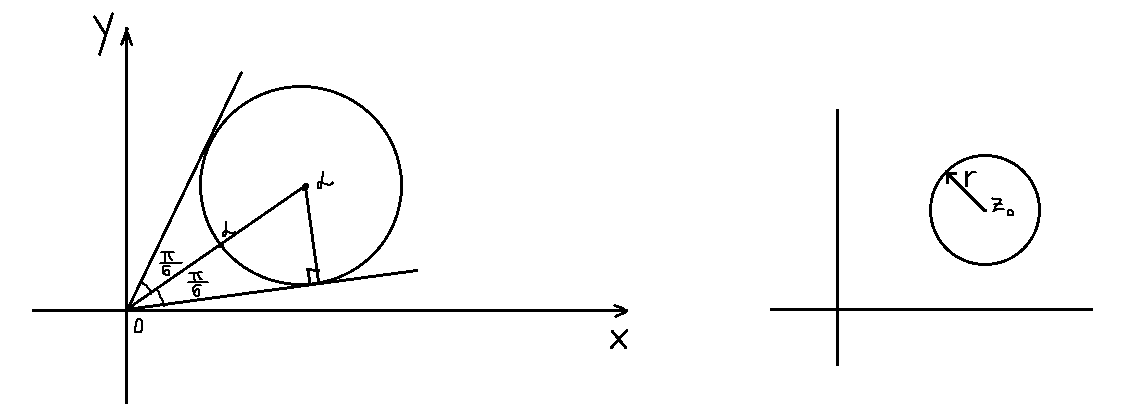
\includegraphics[width=0.74\textwidth]{images/lec2_1.png}
    \end{center}
    Тогда если $z = z_0 + re^{i\phi}$, где $r = |z|$, $e^{i\phi} = \cos(\phi) + i\sin(\phi)$, то справедливо $$arg \left( e^{ip\phi} \left( \alpha + \frac {o((z-z_0))^p}{(z-z_0)^p}\right) \right) = p\phi + \alpha_0 + \beta \frac {\pi}{3}, \ 0 \leq \beta \leq 1.$$
    Так как $\phi$ -- любое вещественное число, то теорема доказана.
\end{proof}

\begin{theorem}[Основная теорема алгебры]
    \label{ota}
    Всякий многочлен положительной степени из кольца $\Cm[x]$ имеет хотя бы один корень, в общем случае комплексный.
\end{theorem}

\begin{proof}
    Пусть $f(x)$ -- многочлены положительной степени. Пусть $A = \inf|f(z)|$, $z \in \Cm$. Покажем, что инфимум достигается, то есть существует такое комплексное $z_n \in \Cm$, что $|f(z_n)| = A$. По определению инфимума существует последовательность ${z_n}$ такая, что её модуль стремится к конечному $A$. Из этой последовательности можно извлечь
    подпоследовательность ${z_{n_k}}$ такую, что она сходится к $z_0$ или к бесконечности. Однако второй случай не реализуется, так как иначе $|f(z_{n_k})|$ также сходится к бесконечности. Тогда $\exists \lim_{k\to \infty} {z_{n_k}} = z_0$, откуда $\exists \lim_{k\to \infty} {f(z_{n_k})} = f(z_0)$, а значит, существует предел модуля такой функции, равный $\lim_{k\to \infty} {|f(z_{n_k})|} = |f(z_0)| = A$. Если оказалось так, что $A \neq 0$, то по лемме Д'Аламбера найдется $z \in U_{\epsilon}(z)$ такой что $|f(x)| < |f(z_0)| = A = \inf(|f(z)|)$, что противоречит определению инфимума. Значит, $A = 0$ и $\exists z_{0}: |f(z_{0})| = 0 \Rightarrow f(z_{0}) = 0$.
\end{proof}